% Created 2023-04-12 Wed 12:24
% Intended LaTeX compiler: pdflatex
\documentclass[11pt]{article}
\usepackage[utf8]{inputenc}
\usepackage[T1]{fontenc}
\usepackage{graphicx}
\usepackage{longtable}
\usepackage{wrapfig}
\usepackage{rotating}
\usepackage[normalem]{ulem}
\usepackage{amsmath}
\usepackage{amssymb}
\usepackage{capt-of}
\usepackage{hyperref}
\author{Antonio Petrillo}
\date{\today}
\title{Easter Exercise}
\hypersetup{
 pdfauthor={Antonio Petrillo},
 pdftitle={Easter Exercise},
 pdfkeywords={},
 pdfsubject={},
 pdfcreator={Emacs 29.0.60 (Org mode 9.6.1)}, 
 pdflang={English}}
\begin{document}

\maketitle
\tableofcontents


\section{Esercizio 1}
\label{sec:org7d35040}
Implementare WeightedSet.
\begin{verbatim}
import java.util.Iterator;
import java.util.SortedSet;
import java.util.TreeSet;

public class MyWeightedSet<T> {

    private static class Entry<E> implements Comparable<Entry<?>> {
        E element;
        Integer weight;

        Entry(E element, Integer weight) {
            this.element = element;
            this.weight = weight;
        }

        @Override
        public int compareTo(Entry<?> other) {
            return Integer.compare(weight, other.weight);
        }

        @Override
        public String toString() {
            return element.toString();
        }
    }

    private SortedSet<Entry<T>> set;
    private Integer threshold;

    public MyWeightedSet() {
        this.set = new TreeSet<>();
        this.threshold = null;
    }

    private boolean checkThreshold(Integer weight) {
        return threshold == null || threshold != null && weight >= threshold;
    }

    public boolean add(T t, Integer weight) {
        Entry<T> e = new Entry<>(t, weight);
        if (checkThreshold(weight)) {
            if (set.contains(e)) {
                set.remove(e);
                // questa parte é un pó strana ma l'esempio del caso d'uso
                // fa vedere che l'Entry (new Object, 5) viene sostituita da ("Jesse", 5)
                // usando il normale add di SortedSet sarei ("Jesse", 5) non verrebbe mai
                // aggiunto
            }
            return set.add(e);
        }
        return false;
    }

    private MyWeightedSet(SortedSet<Entry<T>> set, Integer threshold) {
        this.set = set;
        this.threshold = threshold;
    }

    public MyWeightedSet<T> atLeast(Integer threshold) {
        return new MyWeightedSet<T>(set, threshold);
    }

    @Override
    public String toString() {
        StringBuilder sb = new StringBuilder();
        sb.append("[");
        Iterator<? extends Entry<?>> iter = set.iterator();
        while (iter.hasNext()) {
            Entry<?> e = iter.next();
            if (checkThreshold(e.weight)) {
                sb.append(e);
                if (iter.hasNext()) {
                    sb.append(", ");
                }
            }
        }
        sb.append("]");
        return sb.toString();
    }

    // sed -i -e '90s/ar/er/g' MyWeightedSet.java
    public static void main(String[] args) {
        MyWeightedSet<Object> set = new MyWeightedSet<>();
        set.add(Double.valueOf(3.14), 100);
        set.add(new Object(), 5);
        set.add("Skylar", 50);
        set.add("Jesse", 5);
        System.out.println(set);
        MyWeightedSet<Object> set10 = set.atLeast(10);
        System.out.println(set10);
        set.add("Walter", 60);
        System.out.println(set);
        System.out.println(set10);
    }
}
\end{verbatim}
\subsection{Note}
\label{sec:org2b2dfa2}
I motivi principali per cui \texttt{WeightedSet} non estende \texttt{Set} sono:
\begin{enumerate}
\item troppi metodi non richiesti da implementare
\item il metodo \texttt{add} di Set non é compatibile con il caso d'uso dell'esempio
\end{enumerate}

Sempre nel metodo \texttt{add}, come si evince dal caso d'uso, nel momento in cui viene aggiunto un nuovo oggetto, chiamiamolo \texttt{A}, con un valore giá presente, chiamiamolo \texttt{B}, allora \texttt{A} dovrá sostituire \texttt{B}.
Questo é il motivo per cui il metodo add fa ulteriori controlli.
Ció puó essere visto nel caso d'uso, \texttt{set.add(new Object(), 5)} viene sostituito da \texttt{set.add("Jesse", 5)}.
\section{Esercizio 2}
\label{sec:org7c84f6e}
Dato l'interfaccia:
\begin{verbatim}
interface Predicate<T> {
    boolean test(T t);
}
\end{verbatim}
Dire quali dei seguenti contratti per un \uline{comparatore} di \texttt{Predicate} sono validi.
\subsection{Contratto a}
\label{sec:org3b5a414}
\(-1\) se \texttt{x.test(...)} sempre falso e \texttt{y.test(...)} sempre vero.
\(1\) se \texttt{y.test(...)} sempre falso e \texttt{x.test(...)} sempre vero.
\subsubsection{Risposta}
\label{sec:org29077a0}
Il contratto non é valido, non é transitivo.
Supponiamo \(x,y,z\) tali che \texttt{compare(x,y) => -1} e \texttt{compare(y,z) => -1} dovremmo avere che \texttt{compare(x,z) => -1} ma questo non é garantito dalla specifica.
\subsection{Contratto b}
\label{sec:org5584f2e}
\(-1\) se per tutti gli oggetti t il valore di  \texttt{x.test(t)} é l'opposto di \texttt{y.test(t)}.
\(1\) se per tutti gli oggetti t il valore di  \texttt{x.test(t)} é uguale di \texttt{y.test(t)}.
\subsubsection{Risposta}
\label{sec:orgf2d2477}
Il contratto non é valido, in particolare non é antisimmetrico.
Consideriamo il seguente caso:
Prendiamo \texttt{x, y} tale che \texttt{x.test(t) == ! y.test(t)} per un qualche \texttt{t}.
In questo caso il contratto specifica che \texttt{x.test(t) == !y.test(t)} produce \texttt{-1}.
Invertendo l'ordine di x e y si ha:
\texttt{y.test(t) == !x.test(t)} che produce sempre \texttt{-1} e non \texttt{1}, questo perché se é vero che \texttt{x.test(t)} produce sempre un valore opposto a \texttt{y.test(t)} é anche vero il contrario.
\subsection{Contratto c}
\label{sec:orgde7a16e}
\(-1\) se l'insieme degli oggetti t per cui \texttt{x.test(t)} restituisce vero é un sottoinsieme proprio dell'insieme degli oggetti per cui \texttt{y.test(t)} restitituisce vero.
\(1\) se esiste un oggetto t tale che \texttt{x.test(t)} restituisce vero e \texttt{y.test(t)} restituisce falso.
\subsubsection{Risposta}
\label{sec:org9be0948}
Il contratto é valido
\subsection{Contratto d}
\label{sec:org991dbb1}
\(-1\) se ci sono almeno 10 oggetti diversi su cui \texttt{x.test(t)} restituisce vero e \texttt{y.test(t)} restituisce falso.
\(1\) se ci sono almeno 10 oggetti diversi su cui \texttt{x.test(t)} restituisce false e \texttt{y.test(t)} restituisce vero.
\subsubsection{Risposta}
\label{sec:org4aca544}
Il contratto é non valido, in particolare non é transitivo.
Supponiamo di avere \(3\) istanze \(x, y, z\) tali che ci sono:
Almeno 10 elementi \(t_i\) tali che \(x.test(t_i)\) sia vero e \(y.test(t_i)\) sia falso, inoltre ci sono almeno altri 10 elementi \(k_i\) tali che \(y.test(k_i)\) sia vero e \(z.test(k_i)\) sia falso.
Per le specifiche di comparable ci aspetteremmo che \texttt{compare(x, z) == -1}, ma nessuno garantisce che esistano 10 elementi \(v_i\) per cui \(x.test(v_i)\) sia vero e \(z.test(v_i)\) sia falso.
\section{Esercizio 3}
\label{sec:org30642d0}
Data la classe:
\begin{verbatim}
public class A {

    private A other;

    public A(A other) {
        this . other = other;
    }

public class B {
    private static int counter = 0;
    private int id = counter++;
}

    public Object makeObj(int val) {
        return new B() { private int j = val ;};
    }
}
\end{verbatim}
Ed il seguente snippet:
\begin{verbatim}
A a1 = new A(null);
A a2 = new A(a1);
A.B b = a1.new B();
Object x = a1.makeObj(42);
A.B y = (A.B) a2.makeObj(42);
\end{verbatim}
Disegnare il memory layout
\subsection{Memory layout}
\label{sec:orgdbf6aad}
\begin{itemize}
\item a1.other -> null
\item a2.other -> a1
\item b1.id = 1
\item b1.A.this -> a1
\item x.id = 2
\item x.j = 42
\item x.A.this -> a1
\item y.id = 1
\item y.j = 42
\item y.A.this -> a2
\end{itemize}
\subsection{Graficamente}
\label{sec:org3863a57}
\begin{center}
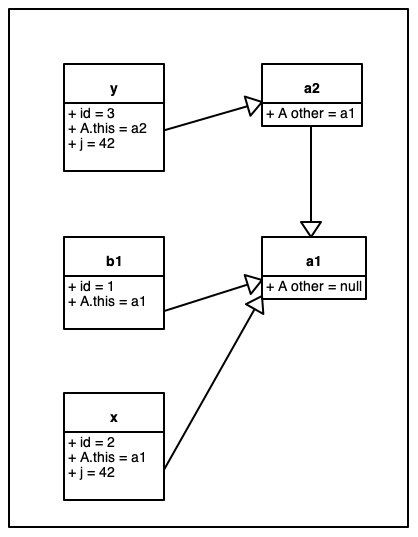
\includegraphics[width=.9\linewidth]{./src/mem_layout.png}
\end{center}
\section{Esercizio 4}
\label{sec:org93650b8}
\begin{center}
\begin{tabular}{ll}
Question & Answer\\[0pt]
\hline
AR<Int> subtype of L<? ext Num> & True\\[0pt]
Set<? ext Num> subtype of Set<? sup Num> & False\\[0pt]
Map<Str, ? ext Num> subtype of Map<Object, ?> & False\\[0pt]
TreeSet<Integer> subtype of SortedSet<? super Integer> & True\\[0pt]
HashMap<Integer, Double> subtype of Map<?, ? super Double> & True\\[0pt]
\end{tabular}
\end{center}
\end{document}